\documentclass[a4paper,12pt]{article}
\usepackage{times}
\usepackage[pdftex]{graphicx,color}
\graphicspath{{fig/}}
\usepackage[colorlinks=false,pdfborder=000]{hyperref}
\usepackage{enumerate}
\usepackage{multirow}
\usepackage{titling}
\usepackage[top=1.2in, bottom=1.2in, left=1.2in, right=1.2in]{geometry}
\usepackage{comment}
\usepackage{indentfirst}
\usepackage{amsmath}

%%%%%%%%%%%%%%%%%%%%%%%%%%%%%%%%%%%%%%%%%%%%%%%%%%%%%%%%%%%%%%%%%%%%%%%%%%%%%%%%%%%%%%%%%%%%%%%%%%%%%%%%%%%%%%%%%%%%%%%%%%%%
\newcommand{\CSE}{\href{http://www.cse.cuhk.edu.hk}{Department of Computer Science and
Engineering}}
\newcommand{\CUHK}{\href{http://www.cuhk.edu.hk}{The Chinese University of Hong Kong}}
\newcommand{\mymail}{\mbox{\textcolor{blue}{\underline{zgxiao@cse.cuhk.edu.hk}}}}
\newcommand{\myname}{\href{http://www.cse.cuhk.edu.hk/~zgxiao}{XIAO Zigang}}
\newcommand{\header}[1]{\noindent {\bf \\#1\\}}
\newcommand{\NE}{Nash Equilibrium }
\newcommand{\tot}{\frac{2}{3}}
%%%%%%%%%%%%%%%%%%%%%%%%%%%%%%%%%%%%%%%%%%%%%%%%%%%%%%%%%%%%%%%%%%

% modify the font size of title, author and date
\pretitle{\begin{center}\bf \Huge} \posttitle{\par\end{center}}
\preauthor{\begin{center}
            \small \small \lineskip 0.5em%
            \begin{tabular}[t]{c}}
\postauthor{\end{tabular}\par\end{center}}
\predate{\begin{center}\small} \postdate{\par\end{center}}

\title{CSC5240 Project Report\\\Large Droplet Manipulation in Cross-Referencing Digital Microfluidic Biochip}
\author{\myname\\\mymail\\\CSE\\\CUHK}
\date{\today}

%%%%%%%%%%%%%%%%%%%%%%%%%%%%%%%%%%%%%%%%%%%%%%%%%%%%%%%%%%%%%%%%%%
\begin{document}
\bibliographystyle{unsrt}
\maketitle
\abstract{Digital Microfluidic Biochip (DMFB) has drawn lots of attention nowadays,
 especially the \textit{cross-referencing biochip}.
Due to electrode constraint, the manipulation of droplets to avoid electrode interference becomes crucial in droplet routing.
This project tries to solve this problem by using constraint satisfaction technique.
}
%%%%%%%%%%%%%%%%%%%%%%%%%%%%%%%%%%%%%%%%%%%%%%%%%%%%%%%%%%%%%%%%%%
\section{Background}
Digital Microfluidic Biochip has been receiving more and more attention nowadays.
It is crucial in medical, pharmaceutical and environmental monitoring applications \cite{verpoorte2003mmm}.
The discrete objects we want to operate on chip are called \textit{droplets}.
They are the carriers of biochemical materials that we want to perform operation with.
Analogous to VLSI synthesis, a top-down approach can be applied to biochip design,
and \textit{droplet routing} is one of the important steps in biochip synthesis(Figure \ref{fig:dmfb}).
\begin{figure}[!htbp]
\centering
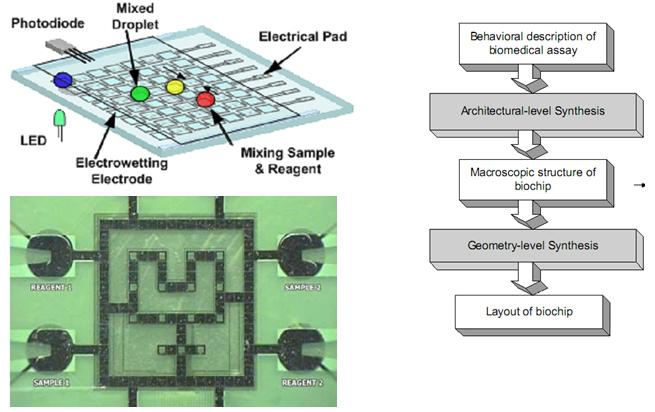
\includegraphics[width=0.6\textwidth]{dmfb.jpg}
\caption{DMFB and its top-down design methodology}
\label{fig:dmfb}
\end{figure}
The goal is to route a set of droplets from their \textit{source} to their \textit{sink}.
Figure \ref{fig:routing} gives an illustration.
\begin{figure}[!htbp]
\centering
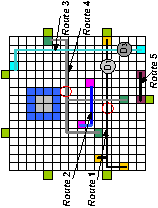
\includegraphics[angle=-90,width=0.3\textwidth]{routing}
\caption{Droplet Routing}
\label{fig:routing}
\end{figure}

Currently, there exist two kinds of techniques to manipulate droplets movement.
The first one is \textit{direct-addressing},
in which an electrode is fixed under each cell of the chip.
It is simple, yet expensive and rather limited for large scale product.
Another more promising method is \textit{cross-referencing},
which applies high/low voltage to a row electrode and a column electrode
in order to activate the cell in their intersection point, as in Figure \ref{fig:highlow}.
\begin{figure}[!htbp]
\centering
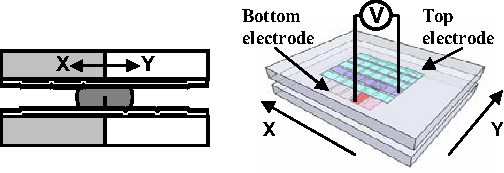
\includegraphics[width=0.4\textwidth]{highlow}
\caption{Cross-referencing manipulation scheme}
\label{fig:highlow}
\end{figure}
However, because the activation of a cell is in a row-column manner,
which means \textit{extra cells} may be activated when multiple rows/columns are addressed.
We call it \textit{electrode interference} and it imposes \textit{electrode constraint} on droplet routing.
Figure \ref{fig:eleinter} shows this situation.
\begin{figure}[!htbp]
\centering
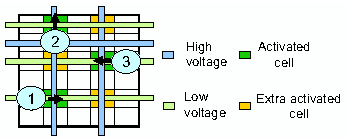
\includegraphics[width=0.4\textwidth]{eleinter}
\caption{Electrode Interference to droplet 2}
\label{fig:eleinter}
\end{figure}
The objective of \textit{Droplet Routing and Manipulation in Cross-Referencing Digital Microfluidic Biochip}
is to route the droplets and minimize the droplet routing time while not violating the electrode constraint.


\section{Literature Review}
The earliest article about droplet routing problem can be found in \cite{bohringer2003osm},
in which the author used a \textit{robotic} viewpoint to solve routing.
\cite{bohringer2006mac}\cite{1326232}\cite{1353672} use \textit{$A*$ search,network flow} and \textit{bypassibility} heuristic to generate routes.
However, none of them considered cross-referencing.
Cross-referencing routing is first considered in \cite{bohringer2003osm},but no concrete algorithm is given.
Currently there are only three papers handle droplet routing and cross-referencing manipulation at the same time.
\cite{griffith2006pcr} reduces the problem to a \textit{graph-coloring} problem.
\cite{1266484} transform the problem to a \textit{maximum clique partition} problem.
Both of them first found a solution for direct-addressing biochip and transform the solution to adapt cross-referencing,
by splitting each step in direct-addressing in to several steps so that no violation will be caused.
\cite{yuh2008pib} first deals with the problem directly from a cross-referencing biochip assumption,
i.e. he treat the problem as a whole and tries to route the droplets while at the same time considering the cross-referencing constraint.
More specifically, it uses a \textit{progressive linear programming} with heuristic at each step to get a near-optimal solution.

\section{Problem Formulation}
There is a \text{route} for each droplet. Nevertheless,
these routes are \textit{virtual routes} which are different from those in VLSI design,
since they can \textit{intersect} with each other,
and we only need to ensure the droplets would not ``crash'' each other at the intersection point.

Each droplet can be interpreted as a moving robot.
Then the routing problem can be reduced to \textit{motion planning} problem in robotics research.
It is proved to be NP-hard by Erdmann et al.\cite{erdmannmovingobj}.

Moreover, because of \textit{electrode interference},
it is almost impossible to accomplish the parallel moving of droplet, which can be easily achieved in direct-addressing biochip.
In this project we are going to explore the possibility of solving this problem by using \textit{constraint programming} technique.

The problem can be given as:
\textit{Given a snapshot during droplet routing, find a correct voltage assignment schedule, while minimizing the total time used,}
where a series of snapshots could be obtained from direct-addressing result.
Figure \ref{fig:clique} gives an example of \textit{snapshot}.
\begin{figure}[!htbp]
\centering
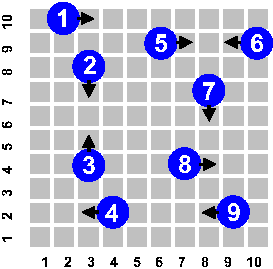
\includegraphics[width=0.3\textwidth]{clique}
\caption{Example of a snapshot. $10\times10$ biochip with 9 droplets on it.
The arrow denotes the moving direction of each droplet.}
\label{fig:clique}
\end{figure}
\begin{itemize}
  \item
        A snapshot consists of:
        \begin{itemize}
        \item N rows and M columns
        \item n droplets denoted by adjacent start and end location
        \end{itemize}
  \item A voltage assignment schedule is:
        \begin{itemize}
          \item At time step t, the voltage on each row/column
        \end{itemize}
\end{itemize}

\section{Modeling}
\subsection{Constraints}
\begin{itemize}
  \item Fluidic Constraint\\
  At any time, droplets can not be mixed together.
  Hence there should be at least one spacing between each droplet.
  \item Timing Constraint\\
  All droplet must be moved within time $T$.
  \item Electrode Constraint\\
  While activating some electrodes simultaneously, no interference is caused.
\end{itemize}

\subsection{Modeling Consideration}
First we should note that with or without careful voltage assignment,
we can avoid electrode interference to a certain extent.
Figure \ref{fig:careful} is an example from \cite{1189844}.
The figure shows that there are two droplets on a chip.
For the second picture, two cells are activated between either droplet.
Then it causes electrode interference(the droplet may be unexpectedly split).
However, by assigning voltage as in the last picture,
no extra activated cell will be caused.

\begin{figure}[!htbp]
\centering
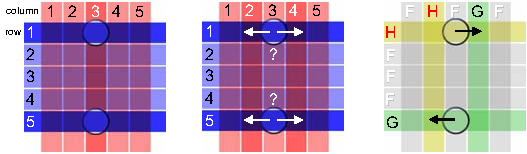
\includegraphics[width=0.5\textwidth]{careful}
\caption{Avoiding electrode constraint}
\label{fig:careful}
\end{figure}

Second, we need to consider the granularity of cells.
Suppose a droplet moves at time $t$, then before time $t$,
all the 8 neighboring cells around the start location can no be activated.
But after time $t$ it moves to the end location,
then 8 neighboring cells around the end location can not be activated now.
Below is an illustration:

\begin{figure}[!htbp]
\centering
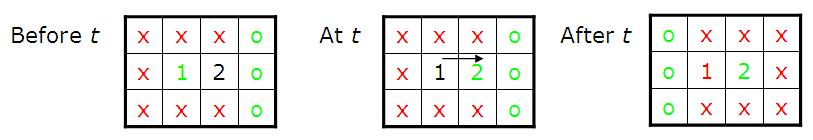
\includegraphics[width=0.6\textwidth]{criticalarea.jpg}
\label{fig:criticalarea}
\end{figure}

Next, we have to decide whether we take `merge' into account or not.
Mixing operation may need two droplets be mixed together,
then route to their destination.
If we do not consider this special case, then this situation will be considered as invalid.
Below is an illustration:

\begin{figure}[!htbp]
\centering
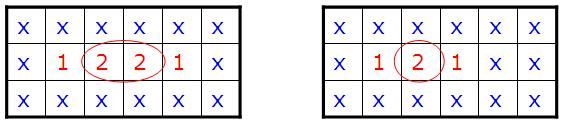
\includegraphics[width=0.6\textwidth]{merge.jpg}
\label{fig:merge}
\end{figure}

At last, one very rare case is noted.
A droplet may be moved several times between its start and end location.
But the result is correct if and only if after the maximum time, it stays at end location.
However, since it is too complicated to be taken into account, we do not deal with this case.

\subsection{A Simple Model}
We first build a simple model. The voltage available to row is in \{High,Float\},
and \{Low,Float\} for column, i.e. no flexible voltage assignment be considered.
Also, the delicate granularity will not be considered in this model.

\begin{table}[!htbp]
\centering
\begin{tabular}{|p{.8\linewidth}|}
\hline
\textbf{\color{blue}Variables:} $d_1 \ldots d_n , T$\\
\textbf{\color{blue}Domains:} $d_i \in [1..n] , T\in[1..n]$\\
\textbf{\color{blue}Constraints:}
\begin{itemize}
  \item $d_i \le T$
  \item If $d_i == d_j $ Then corresponding cells would be activated.
  \item If a cell is activated, it will not cause fluidic constraint.
\end{itemize}
\textbf{\color{blue}Objective:} minimize $T$\\
\hline
\end{tabular}
\end{table}

Experimental result is shown in next section.

\subsection{Another Model}
This time we will take flexible voltage assignment into account to see if we can get a better result.

\begin{table}[!htbp]
\centering
\begin{tabular}{|p{.8\linewidth}|}
\hline
\textbf{\color{blue}(new) Variables:}\\
$volRow_{1t},��, volRow_{Nt}$ : row i's voltage at time t\\
$volCol_{1t},��, volCol_{Mt}$ : column j's voltage at time t\\
\textbf{\color{blue}Domains:} \{HIGH,LOW,FLOAT\}\\
\textbf{\color{blue}Constraints:}
\begin{itemize}
  \item If no `2' at a row/col, set to F
  \item If a `2' at row=r,col=c, activated at time t, then
  \begin{itemize}
    \item $volRow_{rt}$ == HIGH and $volCol_{ct}$ == LOW
    \item $volRow_{rt}$ == LOW  and $volCol_{ct}$ == HIGH
  \end{itemize}
  \item for row=r,col=c at time t, fluidic constraint not violated
  \begin{itemize}
    \item $volRow_{rt}$ == HIGH and $volCol_{ct}$ == LOW
    \item $volRow_{rt}$ == LOW  and $volCol_{ct}$ == HIGH
  \end{itemize}
\end{itemize}\\
\hline
\end{tabular}
\end{table}

\section{Experimental Result}
\subsection{Experiment Setup}
The testing is performed in the server {\tt solar4@cse.cuhk.edu.hk} which equipped with {\tt SunOS} and {\tt ILOG solver 6.0}.
We test the program on two class of cases:
\begin{itemize}
  \item Specific cases extracted in papers
  \item Random test cases
\end{itemize}

\subsection{Specific Case}
We take one case of Figure \ref{fig:clique} for comparison of the two models.
\begin{itemize}
  \item
  Model I: ( format: {\tt time: set of droplets})
  \begin{itemize}
    \item 1:\{1,2,3,4\}
    \item 2:\{5,6\}
    \item 3:\{7,8,9\}
  \end{itemize}
  \item
  Model II: (format: {\tt droplet number: time volRow volCol})
  \begin{itemize}
    \item 1: 1   H L
    \item 2: 1   H L
    \item 3: 1   H L
    \item 4: 1   H L
    \item 5: 1   L H
    \item 6: 1   L H
    \item 7: 2   L H
    \item 8: 2   L H
    \item 9: 2   L H
  \end{itemize}
\end{itemize}
Here we can see that model I can get an optimal of 3 while model II can get an optimal of 2,
because it exploits more parallelism.

Also, for both models, it is for sure that they outperform the greedy method proposed in \cite{1266484}.
Since both models can find a solution at least as good as the greedy algorithm.

\subsection{Random Case}
A random test case generator is made for test purpose.
It can generate a snapshot of $N \times M$ biochip with $D$ droplet, all constraints are satisfied.
Several class of test have been performed to test the model.
Each class consists of 100 test cases.
Average optimum is recorded as the expected value of objective.
Average failure is the fail time over total cases number(100 here).
Failure is defined as the runtime exceeds 60 seconds.

\begin{table}[!htbp]
\centering
\begin{tabular}{|c|c|c|c|c|c|c|c|c|}
\hline
        & \multicolumn{2}{|c|}{10 10 8} & \multicolumn{2}{|c|}{10 10 10} & \multicolumn{2}{|c|}{20 20 10} & \multicolumn{2}{|c|}{20 20 20} \\\hline
        & avg-opt & avg-fail & avg-opt & avg-fail & avg-opt & avg-fail& avg-opt & avg-fail\\\hline
Model I  & 4 &  1\% & 6 &  2\%  & 6 &  2\%  & 8 &  5\% \\\hline
Model II & 2 & 10\% & 3 &  50\% & 3 &  50\% & 7 &  70\% \\\hline

\end{tabular}
\end{table}

From the experimental result, we can see that the simple model works very well actually.
Although the second model can get an expected value better than model I, its failure rate is too high.
I notice that if the second model can not can a model very quickly, it might be trapped in a hard instance.
That is the reason why I set the time limit to only 1 minute.
It is very impractical if the computational time is too long,
since for each droplet routing problem, there usually might be 30-50 snapshots.
Also, we can see that the gross optimality we gained is not too much in Model II,
with an large optimality-time trade off.

\section{Conclusion and Future work}
In this project, constraint satisfaction technique is used to solve the droplet manipulation problem.
The routing algorithm may incorporate such a application to solve the problem.
However, there are still many place for improvement.
More real-world constraint should be taken into account, e.g. the 3-pin net.
Also, there should be better modeling for this problem.
Sophisticated constraints, user-defined constraint might be utilized in the project.

%%%%%%%%%%%%%%%%%%%%%%%%%%%%%%%%%%%%%%%%%%%%%%%%%%%%%%%%%%%%%%%%%%
%%%%%%% End of Document
\bibliography{proposal}
\end{document}
